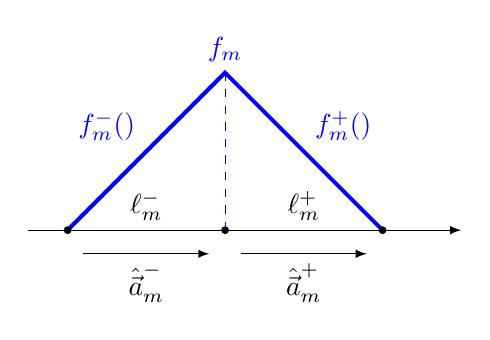
\begin{tikzpicture}[> = latex]
	\draw[->] (-0.5, 0) -- (5, 0);	
	
	\draw[blue, line width=0.5mm] (0, 0) -- node[above left] {$f_m^{-}(\vecr)$} (2, 2) node[above] {$f_m$} -- node[above right] {$f_m^{+}(\vecr)$} (4, 0);
	\draw[blue, dashed] (2, 0) -- (2, 2);
	\node[fill = black, circle, inner sep=0pt, minimum size = 1mm] at (0, 0) {};
	\node[fill = black, circle, inner sep=0pt, minimum size = 1mm] at (2, 0) {};
	\node[fill = black, circle, inner sep=0pt, minimum size = 1mm] at (4, 0) {};
	
	\draw (1, 0) node[above] {$\ell_m^{-}$};
	\draw (3, 0) node[above] {$\ell_m^{+}$};
	
	\draw[->] (0.2, -0.3) -- node[below] {$\hat{\vec{a}}_m^{-}$} (1.8, -0.3);
	\draw[->] (2.2, -0.3) -- node[below] {$\hat{\vec{a}}_m^{+}$} (3.8, -0.3);
\end{tikzpicture}